%% Apêndices

\begin{apendicesenv}
\chapter{Questionário de Pesquisa (Para Gestores)}
\label{apendice:pesquisa-gestores}

Este apêndice apresenta a transcrição do questionário ``Pesquisa para Gestores: Construindo o Novo Sistema de Gestão de Ponto'', desenvolvido na plataforma Google Forms. O instrumento foi aplicado a gestores e proprietários de empresas para mapear os desafios operacionais na gestão da jornada de trabalho e validar as funcionalidades propostas para o sistema.

\section*{Perguntas}
\begin{enumerate}
  \item \textbf{Gostaria de nos informar o nome da sua empresa? (opcional)} \\
        \textit{Campo para resposta curta.}

  \item \textbf{Em qual segmento sua empresa atua?} \\
        \textit{Campo para resposta curta.}

  \item \textbf{Quantos funcionários sua empresa ou equipe possui?} \\
        \textit{Marcar apenas uma oval.}
        \begin{itemize}
          \item 1 - 5
          \item 6 - 10
          \item 11 - 20
          \item Mais de 20
        \end{itemize}

  \item \textbf{Qual é o maior desafio que você enfrenta hoje na gestão do ponto e da jornada de trabalho dos funcionários?} \\
        \textit{Marque todas que se aplicam.}
        \begin{itemize}
          \item Controle de horas extras
          \item Atrasos e faltas frequentes
          \item Integração com contabilidade/folha de pagamento
          \item Processos manuais que tomam muito tempo
          \item Confiabilidade e segurança das marcações
          \item Comunicação com funcionários sobre ajustes e justificativas
          \item Outro
        \end{itemize}

  \item \textbf{Que tipo de sistema você usa atualmente para gerenciar o ponto?} \\
        \textit{Marcar apenas uma oval.}
        \begin{itemize}
          \item Sistema de ponto eletrônico tradicional (REP)
          \item Software/Plataforma online
          \item Planilhas (Excel, Google Sheets)
          \item Processo manual (folhas de ponto em papel)
          \item Nenhum sistema formal
        \end{itemize}

  \item \textbf{De 1 (Dispensável) a 5 (Fundamental), qual a importância de cada uma destas funcionalidades para a gestão da sua equipe?} \\
        \textit{Marcar apenas uma oval por linha.}
        \begin{itemize}
          \item Ter um painel (dashboard) com visão geral do dia (quem está presente/ausente)
          \item Aprovar/rejeitar justificativas de falta (com anexo)
          \item Gerar relatórios de folha de ponto para contabilidade com 1 clique
          \item Fazer ajustes manuais no ponto quando necessário
          \item Configurar diferentes jornadas de trabalho para equipes específicas
          \item Receber alertas sobre inconsistências (ex: horas extras não autorizadas, atrasos)
        \end{itemize}

  \item \textbf{Hoje, qual é o nível de dificuldade para gerenciar o controle de ponto e a jornada de trabalho da sua equipe?} \\
        \textit{Marcar apenas uma oval.}
        \begin{itemize}
          \item Muito fácil – quase não gera problemas
          \item Relativamente fácil – poucas dificuldades no dia a dia
          \item Moderado – exige atenção, mas é gerenciável
          \item Difícil – causa retrabalho e erros frequentes
          \item Muito difícil – é um desafio constante na gestão da equipe
        \end{itemize}

  \item \textbf{Um sistema que automatizasse esse processo e reduzisse erros seria valioso para sua empresa? Por quê?} \\
        \textit{Marcar apenas uma oval.}
        \begin{itemize}
          \item Sim, porque economizaria tempo
          \item Sim, porque reduziria erros e retrabalho
          \item Sim, porque melhoraria a transparência e confiança
          \item Não, já temos um sistema que atende bem
          \item Outro
        \end{itemize}

  \item \textbf{Qual modelo de parceria você consideraria mais justo para usar um sistema completo como este?} \\
        \textit{Marcar apenas uma oval.}
        \begin{itemize}
          \item Uma pequena taxa fixa por mês.
          \item Assinatura mensal por funcionário.
          \item Plano anual.
          \item Não tenho certeza.
        \end{itemize}

  \item \textbf{Você teria interesse em participar de uma demonstração ou de um teste gratuito da plataforma?} \\
        \textit{Marcar apenas uma oval.}
        \begin{itemize}
          \item Sim, quero participar
          \item Talvez, gostaria de receber mais informações
          \item Não tenho interesse no momento
        \end{itemize}
\end{enumerate}

\chapter{Questionário de Pesquisa (Para Funcionários)}
\label{apendice:pesquisa-funcionarios}

Este apêndice apresenta a transcrição do questionário ``Pesquisa: Novo Sistema de Registro de Ponto (Para Funcionários)'', desenvolvido na plataforma Google Forms e aplicado a funcionários de empresas diversas para validar as hipóteses do projeto e levantar os requisitos sob a ótiva do usuário final.

\section*{Perguntas}
\begin{enumerate}
  \item \textbf{Qual é o seu modelo de trabalho atual?} \\
        \textit{Marcar apenas uma oval.}
        \begin{itemize}
          \item Presencial
          \item Híbrido
          \item Remoto
        \end{itemize}

  \item \textbf{Como você registra suas horas de trabalho atualmente?} \\
        \textit{Marcar apenas uma oval.}
        \begin{itemize}
          \item Sistema de ponto eletrônico na empresa (REP)
          \item Aplicativo no celular ou computador
          \item Planilha (Excel, Google Sheets)
          \item Anotação manual (papel, caderno)
          \item Outro
        \end{itemize}

  \item \textbf{Hoje, como você avalia a facilidade de acompanhar e entender todas as suas horas trabalhadas, horas extras...? Você sente que tem acesso completo a essas informações?} \\
        \textit{Marcar apenas uma oval, em uma escala de 1 (Não tenho acesso) a 5 (Tenho acesso completo).}
        \begin{itemize}
          \item 1 \quad 2 \quad 3 \quad 4 \quad 5
        \end{itemize}

  \item \textbf{Qual é a sua maior frustração com o método atual de registrar o ponto?} \\
        \textit{Marcar apenas uma oval.}
        \begin{itemize}
          \item Minha empresa não registra ponto
          \item Nem sempre consigo bater o ponto
          \item Processo é demorado ou complicado
          \item Falta transparência sobre as horas registradas
          \item Erros que precisam ser corrigidos depois
          \item Não consigo justificar faltas ou atrasos pelo sistema atual
          \item Outro
        \end{itemize}

  \item \textbf{De 1 (Irrelevante) a 5 (Essencial), qual a importância de cada uma destas funcionalidades para você em um sistema de ponto?} \\
        \textit{Marcar apenas uma oval por linha.}
        \begin{itemize}
          \item Bater o ponto pelo celular de forma rápida
          \item Acessar um extrato claro das minhas horas trabalhadas
          \item Receber lembretes para não esquecer de bater o ponto
          \item Enviar justificativas (ex: atestados) pelo próprio sistema
          \item Solicitar férias e folgas pelo sistema
          \item Ver o saldo do meu banco de horas atualizado em tempo real
        \end{itemize}

  \item \textbf{Nosso sistema usa a geolocalização do celular para confirmar o local no momento de bater o ponto (as coordenadas só são coletadas no momento do registro). Como você se sentiria sobre isso?} \\
        \textit{Marcar apenas uma oval.}
        \begin{itemize}
          \item Confortável, aumenta a segurança e transparência
          \item Neutro, não me importo
          \item Desconfortável, me preocupo com minha privacidade
        \end{itemize}

  \item \textbf{Você gostaria que sua empresa utilizasse um sistema de registro de ponto digital e que você tivesse acesso às suas horas trabalhadas, horas extras e faltas?} \\
        \textit{Marcar apenas uma oval.}
        \begin{itemize}
          \item Sim, seria útil para acompanhar minhas horas
          \item Talvez, gostaria de receber mais informações
          \item Não vejo necessidade no momento
        \end{itemize}
\end{enumerate}


% respostas do questionário de pesquisa para gestores
\chapter{Respostas do Questionário de Pesquisa (Para Gestores)}
\label{apendice:respostas-gestores}

Este apêndice apresenta os resultados visuais consolidados da pesquisa de mercado qualitativa, obtidos através da plataforma Google Forms. O questionário, detalhado no \autoref{apendice:pesquisa-gestores}, foi aplicado a uma amostragem de duas empresas do setor, com o objetivo de validar as hipóteses do projeto e levantar os requisitos sob a ótica dos gestores. As imagens a seguir correspondem aos gráficos e respostas coletadas para cada pergunta da pesquisa.

% \begin{figure}[h!]
%   \centering
%   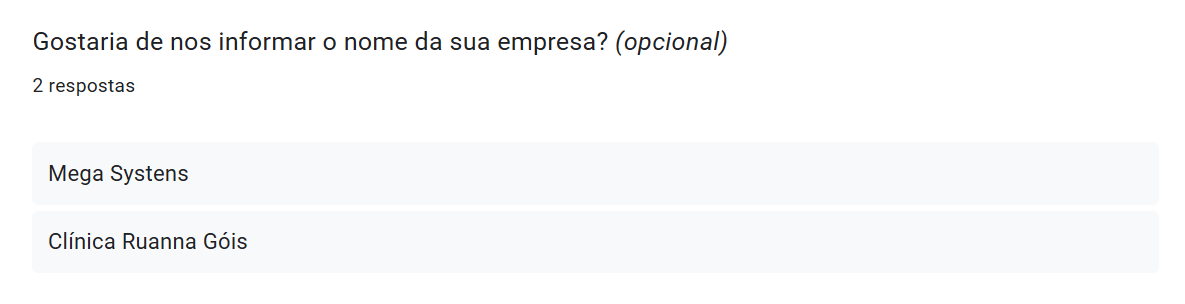
\includegraphics[width=0.8\textwidth]{imagens/nome-empresa.png}
%   \caption{Nome da empresa e segmento de atuação}
%   \label{fig:nome-empresa}
%   \legend{Fonte: Elaborado pela autora (2025).}
% \end{figure}

\begin{figure}[h!]
  \centering
  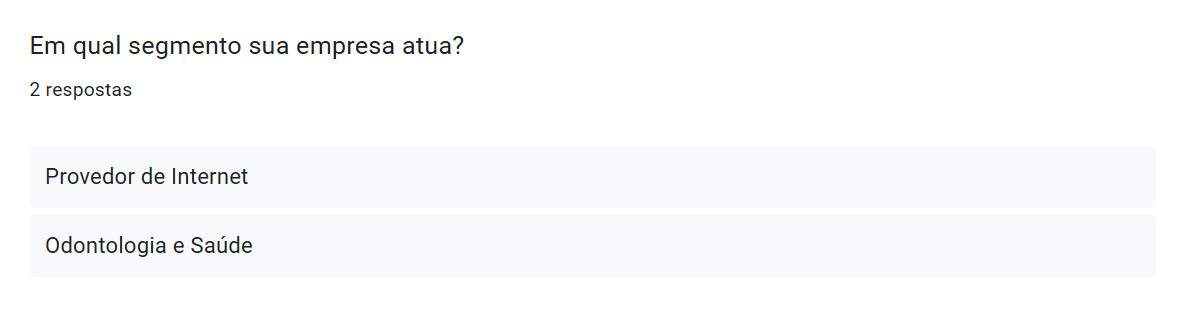
\includegraphics[width=0.8\textwidth]{imagens/segmento.png}
  \caption{Gráfico de respostas para a pergunta: "Em qual segmento sua empresa atua?".}
  \label{fig:resp-gestor-segmento}
  \legend{Fonte: Elaborado pela autora (2025).}
\end{figure}

\begin{figure}[h!]
  \centering
  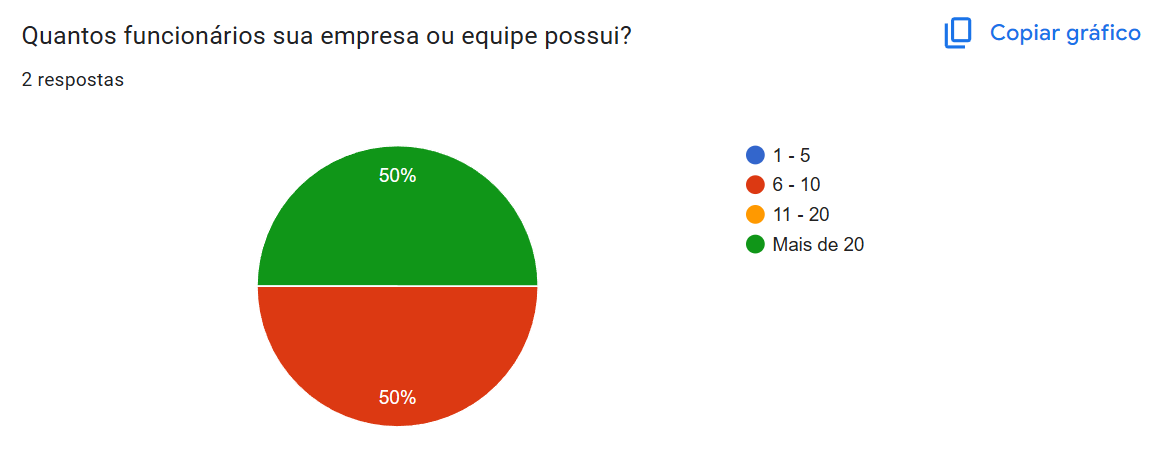
\includegraphics[width=0.7\textwidth]{imagens/quantidade-funcionarios.png}
  \caption{Gráfico de respostas para a pergunta: "Quantos funcionários sua empresa ou equipe possui?".}
  \label{fig:resp-gestor-funcionarios}
  \legend{Fonte: Elaborado pela autora (2025).}
\end{figure}

\begin{figure}[h!]
  \centering
  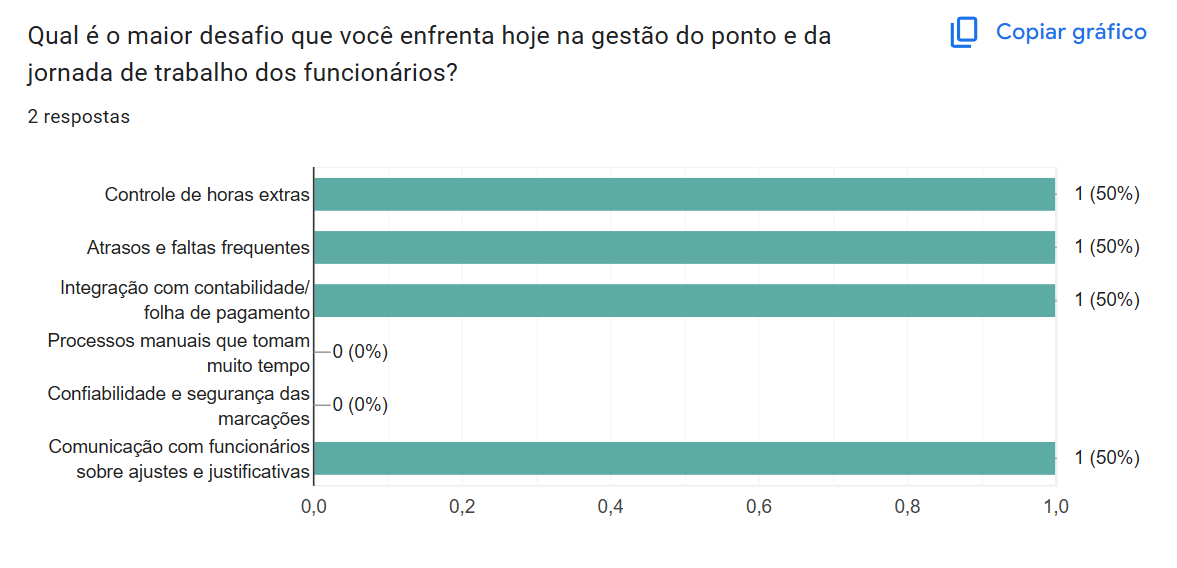
\includegraphics[width=1\textwidth]{imagens/imagem-desafios.png}
  \caption{Gráfico de respostas para a pergunta: "Qual é o maior desafio que você enfrenta hoje na gestão do ponto...?".}
  \label{fig:resp-gestor-desafios}
  \legend{Fonte: Elaborado pela autora (2025).}
\end{figure}

\begin{figure}[h!]
  \centering
  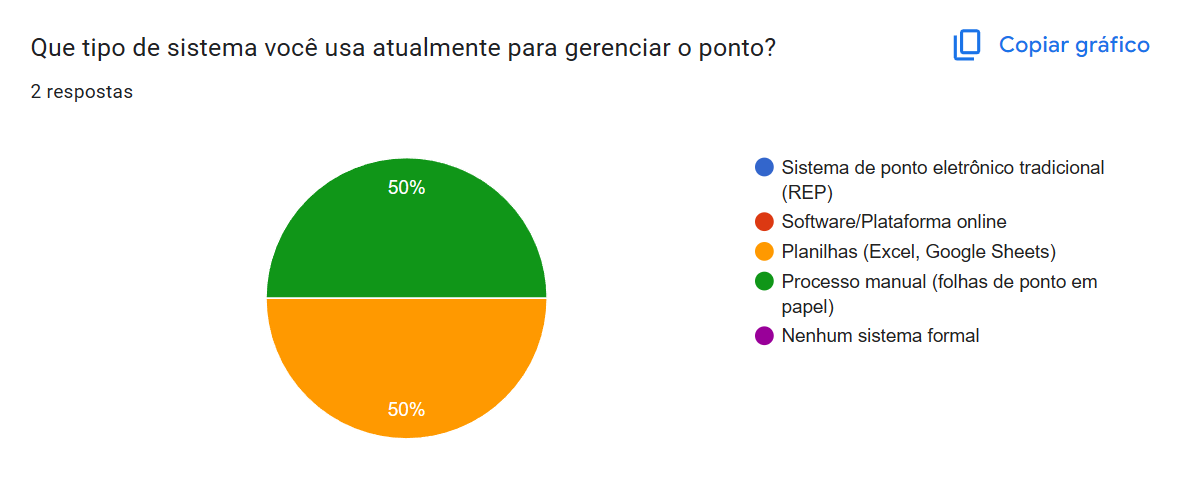
\includegraphics[width=0.7\textwidth]{imagens/imagem_sistema_atual.png}
  \caption{Gráfico de respostas para a pergunta: "Que tipo de sistema você usa atualmente para gerenciar o ponto?".}
  \label{fig:resp-gestor-sistema-atual}
  \legend{Fonte: Elaborado pela autora (2025).}
\end{figure}

\begin{figure}[h!]
  \centering
  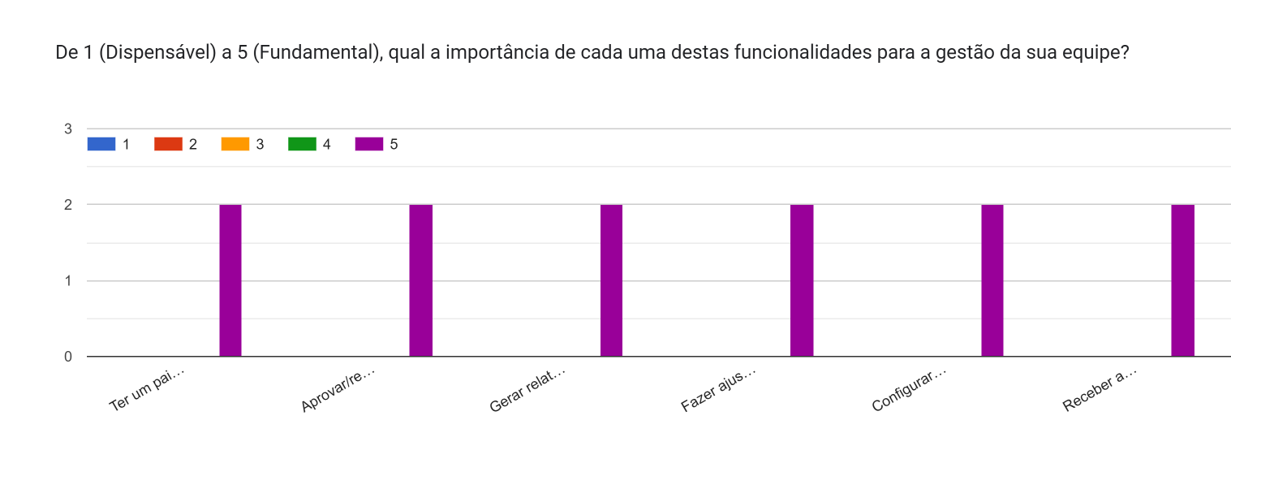
\includegraphics[width=1\textwidth]{imagens/imagem_importancia_func.png}
  \caption{Gráfico de respostas para a pergunta: "De 1 (Dispensável) a 5 (Fundamental), qual a importância de cada uma destas funcionalidades...?".}
  \label{fig:resp-gestor-importancia-func}
  \legend{Fonte: Elaborado pela autora (2025).}
\end{figure}

\begin{figure}[h!]
  \centering
  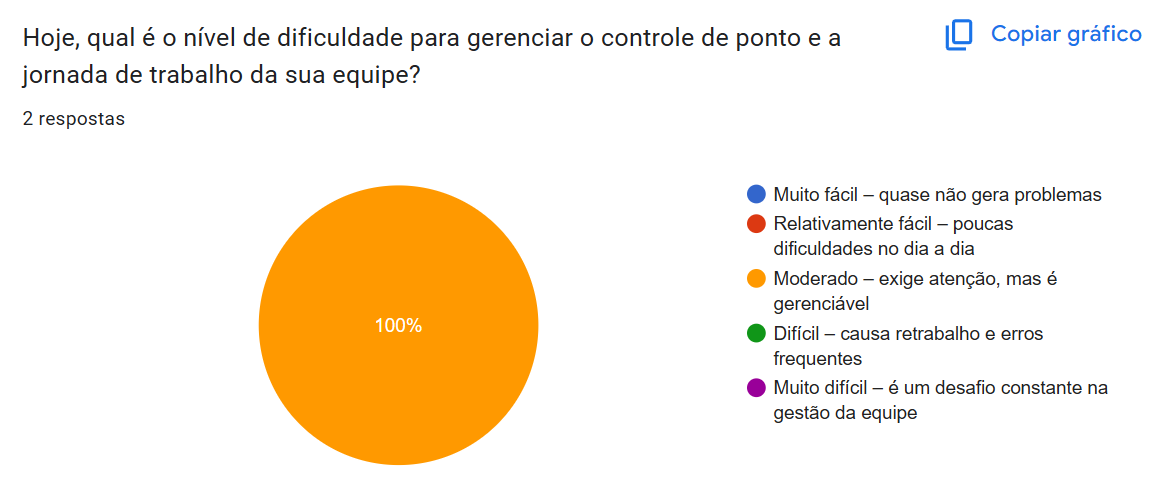
\includegraphics[width=0.7\textwidth]{imagens/imagem-dificuldade.png}
  \caption{Gráfico de respostas para a pergunta: "Hoje, qual é o nível de dificuldade para gerenciar o controle de ponto...?".}
  \label{fig:resp-gestor-dificuldade}
  \legend{Fonte: Elaborado pela autora (2025).}
\end{figure}

\begin{figure}[h!]
  \centering
  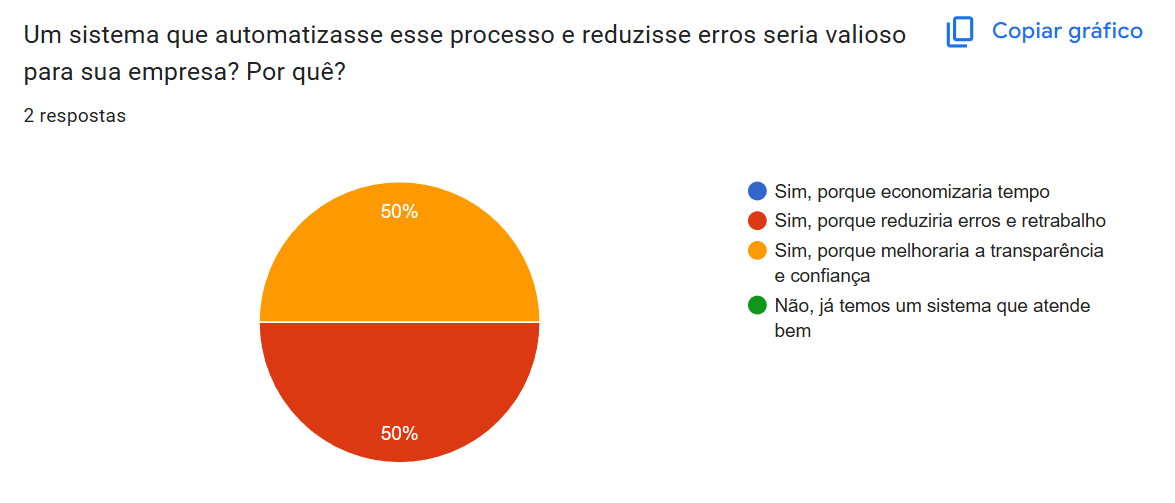
\includegraphics[width=0.8\textwidth]{imagens/imagem_valor_automacao.png}
  \caption{Gráfico de respostas para a pergunta: "Um sistema que automatizasse esse processo e reduzisse erros seria valioso para sua empresa?".}
  \label{fig:resp-gestor-valor-automacao}
  \legend{Fonte: Elaborado pela autora (2025).}
\end{figure}

\begin{figure}[h!]
  \centering
  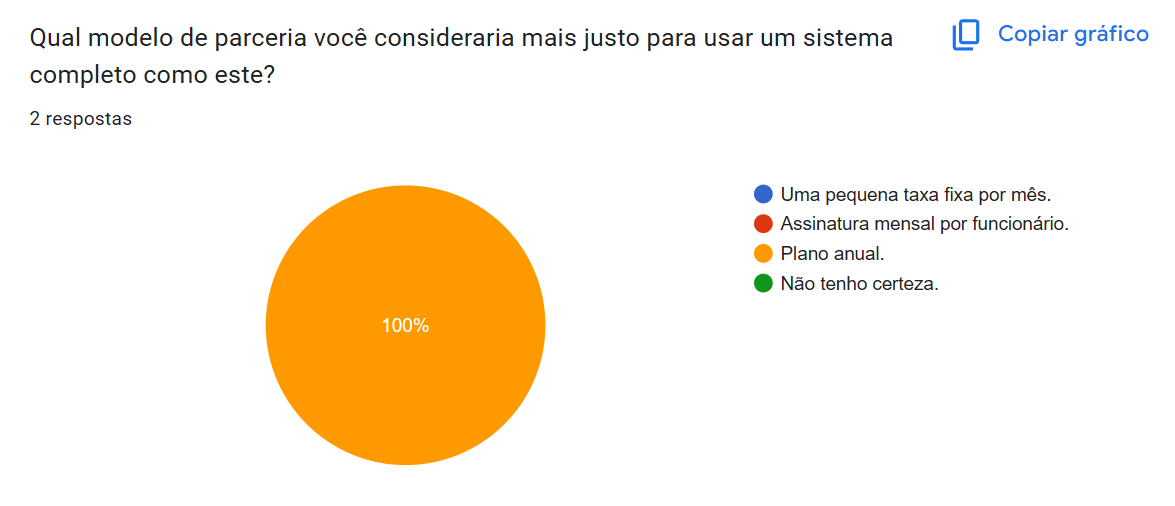
\includegraphics[width=0.7\textwidth]{imagens/parceria.png}
  \caption{Gráfico de respostas para a pergunta: "Qual modelo de parceria você consideraria mais justo...?".}
  \label{fig:resp-gestor-modelo-parceria}
  \legend{Fonte: Elaborado pela autora (2025).}
\end{figure}

\begin{figure}[h!]
  \centering
  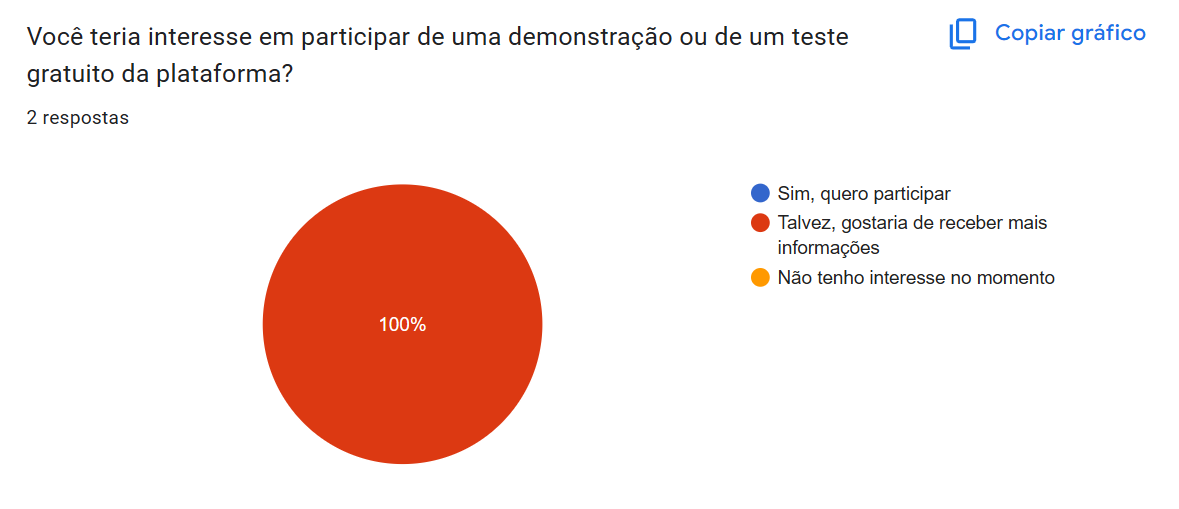
\includegraphics[width=0.7\textwidth]{imagens/interesse-teste.png}
  \caption{Gráfico de respostas para a pergunta: "Você teria interesse em participar de uma demonstração ou de um teste gratuito da plataforma?".}
  \label{fig:resp-gestor-interesse-teste}
  \legend{Fonte: Elaborado pela autora (2025).}
\end{figure}

% respostas do questionário de pesquisa para funcionários
\chapter{Respostas do Questionário de Pesquisa (Para Funcionários)}
\label{apendice:respostas-funcionarios}

Este apêndice apresenta os resultados visuais consolidados da pesquisa de mercado qualitativa com foco nos colaboradores. O questionário, detalhado no \autoref{apendice:pesquisa-funcionarios}, foi respondido por uma amostragem de 31 funcionários de diferentes empresas e setores, com o objetivo de compreender suas percepções e frustrações com os métodos atuais de registro de ponto. As imagens a seguir correspondem aos gráficos e respostas coletadas.

\begin{figure}[h!]
  \centering
  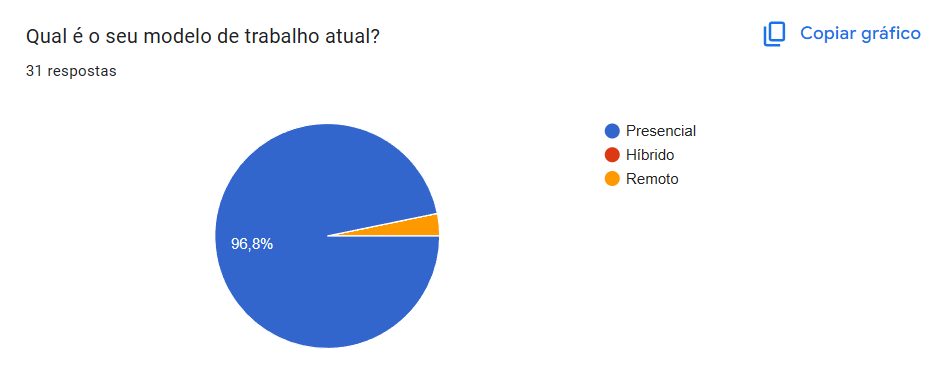
\includegraphics[width=0.7\textwidth]{imagens/modelo-trabalho.png}
  \caption{Gráfico de respostas para a pergunta: "Qual é o seu modelo de trabalho atual?".}
  \label{fig:resp-func-modelo-trabalho}
  \legend{Fonte: Elaborado pela autora (2025).}
\end{figure}

\begin{figure}[h!]
  \centering
  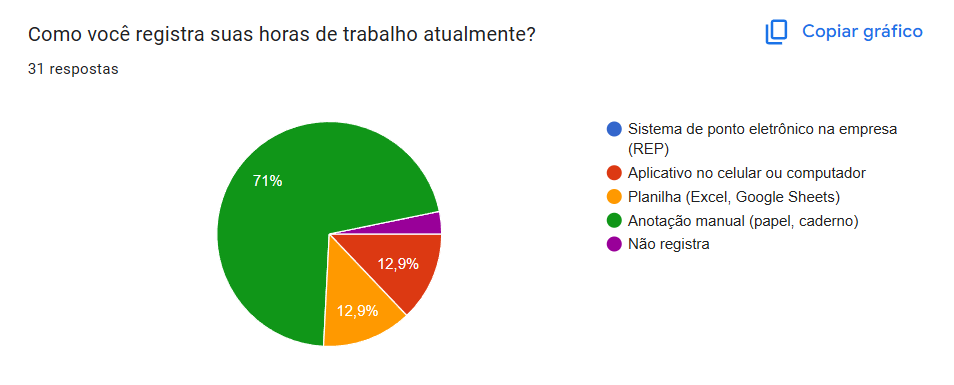
\includegraphics[width=0.7\textwidth]{imagens/como-registra-ponto.png}
  \caption{Gráfico de respostas para a pergunta: "Como você registra suas horas de trabalho atualmente?".}
  \label{fig:resp-func-registro-ponto}
  \legend{Fonte: Elaborado pela autora (2025).}
\end{figure}

\begin{figure}[h!]
  \centering
  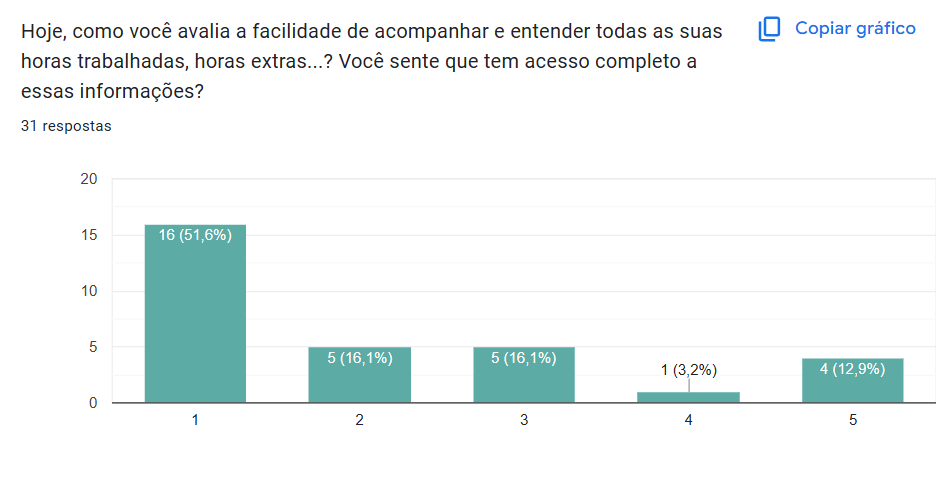
\includegraphics[width=0.7\textwidth]{imagens/como-acompanha.png}
  \caption{Gráfico de respostas para a pergunta: "Hoja, como você avalia a facilidade de acompanhar e entender todas as suas horas trabalhadas, horas extras...? Você sente que tem acesso completo a essas informações?".}
  \label{fig:resp-func-acesso-informacoes}
  \legend{Fonte: Elaborado pela autora (2025).}
\end{figure}

\begin{figure}[h!]
  \centering
  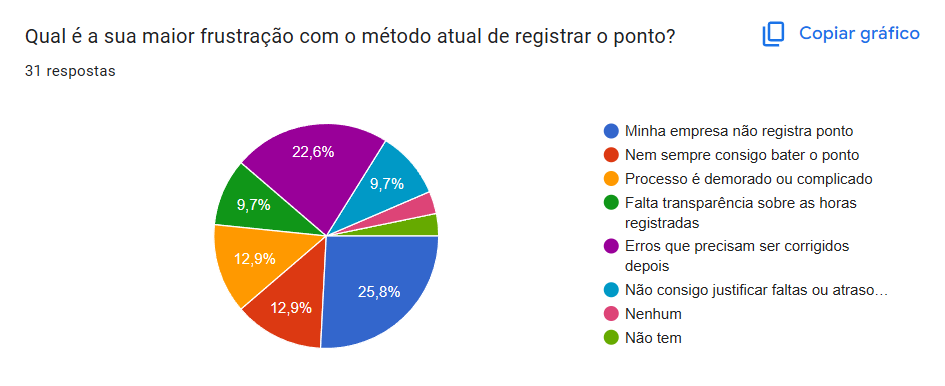
\includegraphics[width=0.7\textwidth]{imagens/maior-frustracao.png}
  \caption{Gráfico de respostas para a pergunta: "Qual é a sua maior frustração com o método atual de registrar o ponto?".}
  \label{fig:resp-func-maior-frustacao}
  \legend{Fonte: Elaborado pela autora (2025).}
\end{figure}

\begin{figure}[h!]
  \centering
  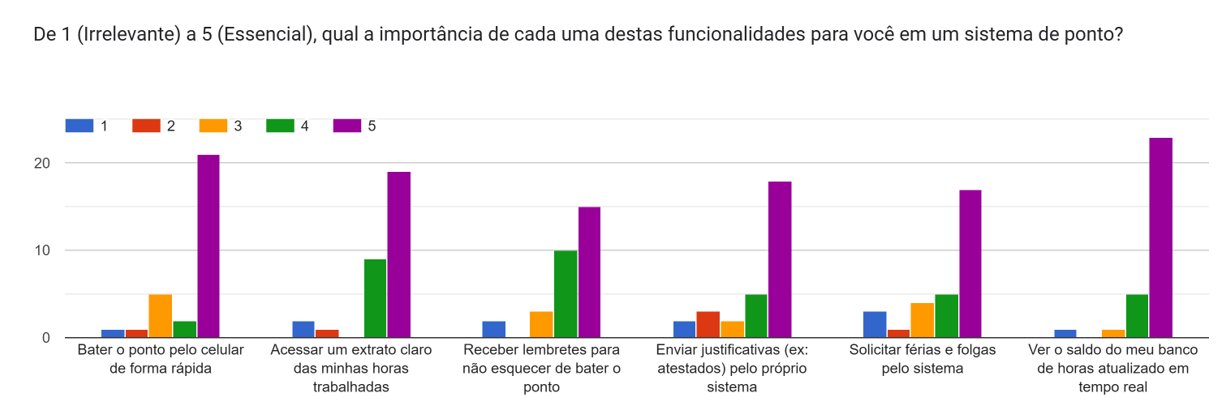
\includegraphics[width=0.7\textwidth]{imagens/importancia-funcionalidades.png}
  \caption{Gráfico de respostas para a pergunta: "De 1 (Irrelevante) a 5 (Essencial), qual a importância de cada uma destas funcionalidades para você em um sistema de ponto?".}
  \label{fig:resp-func-importancia-funcionalidades}
  \legend{Fonte: Elaborado pela autora (2025).}
\end{figure}

\begin{figure}[h!]
  \centering
  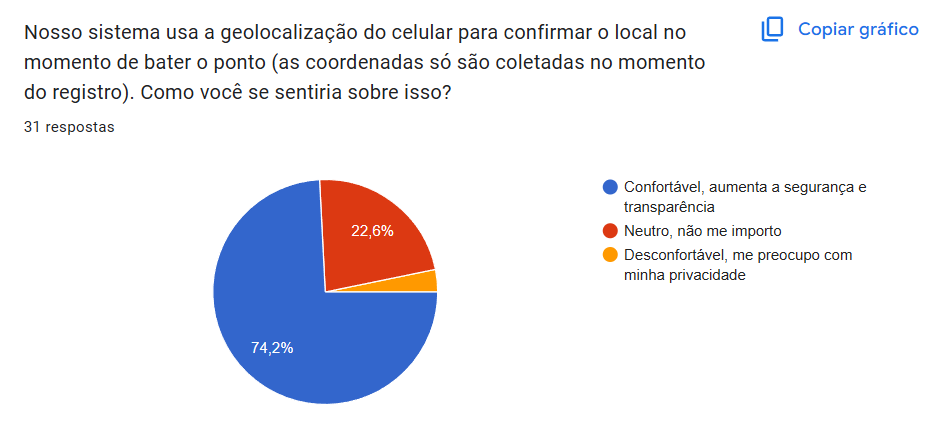
\includegraphics[width=0.7\textwidth]{imagens/geolocalizacao.png}
  \caption{Gráfico de respostas para a pergunta: "Nosso sistema usa a geolocalização do celular para confirmar o local no momento de bater o ponto (as coordenadas só são coletadas no momento do registro). Como você se sentiria sobre isso?".}
  \label{fig:resp-func-geolocalizacao}
  \legend{Fonte: Elaborado pela autora (2025).}
\end{figure}

\begin{figure}[h!]
  \centering
  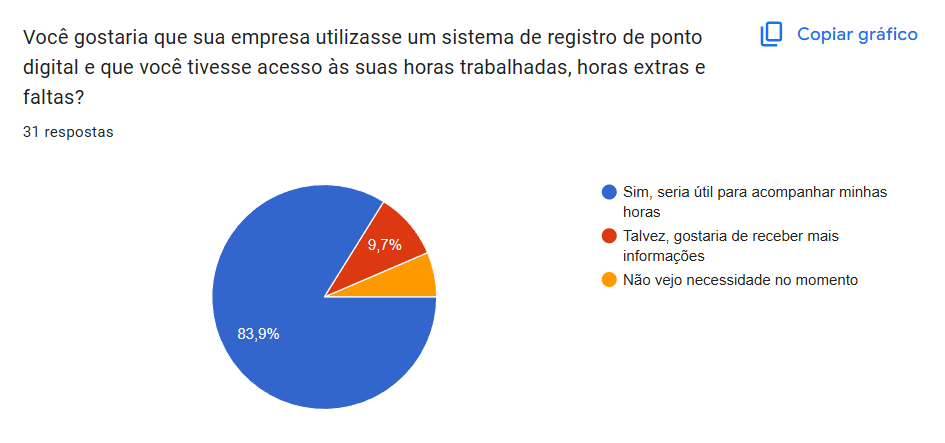
\includegraphics[width=0.7\textwidth]{imagens/interesse-ponto.png}
  \caption{Gráfico de respostas para a pergunta: "Você gostaria que sua empresa utilizasse um sistema de registro de ponto digital e que você tivesse acesso às suas horas trabalhadas, horas extras e faltas?".}
  \label{fig:resp-func-interesse-ponto}
  \legend{Fonte: Elaborado pela autora (2025).}
\end{figure}

\end{apendicesenv}
